\documentclass[twoside]{book}

% Packages required by doxygen
\usepackage{fixltx2e}
\usepackage{calc}
\usepackage{doxygen}
\usepackage{graphicx}
\usepackage[utf8]{inputenc}
\usepackage{makeidx}
\usepackage{multicol}
\usepackage{multirow}
\PassOptionsToPackage{warn}{textcomp}
\usepackage{textcomp}
\usepackage[nointegrals]{wasysym}
\usepackage[table]{xcolor}

% Font selection
\usepackage[T1]{fontenc}
\usepackage{mathptmx}
\usepackage[scaled=.90]{helvet}
\usepackage{courier}
\usepackage{amssymb}
\usepackage{sectsty}
\renewcommand{\familydefault}{\sfdefault}
\allsectionsfont{%
  \fontseries{bc}\selectfont%
  \color{darkgray}%
}
\renewcommand{\DoxyLabelFont}{%
  \fontseries{bc}\selectfont%
  \color{darkgray}%
}
\newcommand{\+}{\discretionary{\mbox{\scriptsize$\hookleftarrow$}}{}{}}

% Page & text layout
\usepackage{geometry}
\geometry{%
  a4paper,%
  top=2.5cm,%
  bottom=2.5cm,%
  left=2.5cm,%
  right=2.5cm%
}
\tolerance=750
\hfuzz=15pt
\hbadness=750
\setlength{\emergencystretch}{15pt}
\setlength{\parindent}{0cm}
\setlength{\parskip}{0.2cm}
\makeatletter
\renewcommand{\paragraph}{%
  \@startsection{paragraph}{4}{0ex}{-1.0ex}{1.0ex}{%
    \normalfont\normalsize\bfseries\SS@parafont%
  }%
}
\renewcommand{\subparagraph}{%
  \@startsection{subparagraph}{5}{0ex}{-1.0ex}{1.0ex}{%
    \normalfont\normalsize\bfseries\SS@subparafont%
  }%
}
\makeatother

% Headers & footers
\usepackage{fancyhdr}
\pagestyle{fancyplain}
\fancyhead[LE]{\fancyplain{}{\bfseries\thepage}}
\fancyhead[CE]{\fancyplain{}{}}
\fancyhead[RE]{\fancyplain{}{\bfseries\leftmark}}
\fancyhead[LO]{\fancyplain{}{\bfseries\rightmark}}
\fancyhead[CO]{\fancyplain{}{}}
\fancyhead[RO]{\fancyplain{}{\bfseries\thepage}}
\fancyfoot[LE]{\fancyplain{}{}}
\fancyfoot[CE]{\fancyplain{}{}}
\fancyfoot[RE]{\fancyplain{}{\bfseries\scriptsize Generated on Thu Sep 18 2014 11\+:55\+:01 for My Project by Doxygen }}
\fancyfoot[LO]{\fancyplain{}{\bfseries\scriptsize Generated on Thu Sep 18 2014 11\+:55\+:01 for My Project by Doxygen }}
\fancyfoot[CO]{\fancyplain{}{}}
\fancyfoot[RO]{\fancyplain{}{}}
\renewcommand{\footrulewidth}{0.4pt}
\renewcommand{\chaptermark}[1]{%
  \markboth{#1}{}%
}
\renewcommand{\sectionmark}[1]{%
  \markright{\thesection\ #1}%
}

% Indices & bibliography
\usepackage{natbib}
\usepackage[titles]{tocloft}
\setcounter{tocdepth}{3}
\setcounter{secnumdepth}{5}
\makeindex

% Hyperlinks (required, but should be loaded last)
\usepackage{ifpdf}
\ifpdf
  \usepackage[pdftex,pagebackref=true]{hyperref}
\else
  \usepackage[ps2pdf,pagebackref=true]{hyperref}
\fi
\hypersetup{%
  colorlinks=true,%
  linkcolor=blue,%
  citecolor=blue,%
  unicode%
}

% Custom commands
\newcommand{\clearemptydoublepage}{%
  \newpage{\pagestyle{empty}\cleardoublepage}%
}


%===== C O N T E N T S =====

\begin{document}

% Titlepage & ToC
\hypersetup{pageanchor=false,
             bookmarks=true,
             bookmarksnumbered=true,
             pdfencoding=unicode
            }
\pagenumbering{roman}
\begin{titlepage}
\vspace*{7cm}
\begin{center}%
{\Large My Project }\\
\vspace*{1cm}
{\large Generated by Doxygen 1.8.8}\\
\vspace*{0.5cm}
{\small Thu Sep 18 2014 11:55:01}\\
\end{center}
\end{titlepage}
\clearemptydoublepage
\tableofcontents
\clearemptydoublepage
\pagenumbering{arabic}
\hypersetup{pageanchor=true}

%--- Begin generated contents ---
\chapter{R\+E\+A\+D\+M\+E}
\label{md__r_e_a_d_m_e}
\hypertarget{md__r_e_a_d_m_e}{}
\input{md__r_e_a_d_m_e}
\chapter{Hierarchical Index}
\section{Class Hierarchy}
This inheritance list is sorted roughly, but not completely, alphabetically\+:\begin{DoxyCompactList}
\item \contentsline{section}{application.\+Chess}{\pageref{classapplication_1_1_chess}}{}
\item \contentsline{section}{application.\+Game}{\pageref{classapplication_1_1_game}}{}
\item \contentsline{section}{application.\+Map}{\pageref{classapplication_1_1_map}}{}
\item \contentsline{section}{application.\+Map\+Tile}{\pageref{classapplication_1_1_map_tile}}{}
\item \contentsline{section}{application.\+Pair}{\pageref{classapplication_1_1_pair}}{}
\item \contentsline{section}{application.\+Piece}{\pageref{classapplication_1_1_piece}}{}
\begin{DoxyCompactList}
\item \contentsline{section}{application.\+Archbishop}{\pageref{classapplication_1_1_archbishop}}{}
\item \contentsline{section}{application.\+Bishop}{\pageref{classapplication_1_1_bishop}}{}
\item \contentsline{section}{application.\+Chancellor}{\pageref{classapplication_1_1_chancellor}}{}
\item \contentsline{section}{application.\+King}{\pageref{classapplication_1_1_king}}{}
\item \contentsline{section}{application.\+Knight}{\pageref{classapplication_1_1_knight}}{}
\item \contentsline{section}{application.\+Pawn}{\pageref{classapplication_1_1_pawn}}{}
\item \contentsline{section}{application.\+Queen}{\pageref{classapplication_1_1_queen}}{}
\item \contentsline{section}{application.\+Rook}{\pageref{classapplication_1_1_rook}}{}
\end{DoxyCompactList}
\item \contentsline{section}{application.\+Player}{\pageref{classapplication_1_1_player}}{}
\item \contentsline{section}{application.\+Test\+Pieces}{\pageref{classapplication_1_1_test_pieces}}{}
\end{DoxyCompactList}

\chapter{Class Index}
\section{Class List}
Here are the classes, structs, unions and interfaces with brief descriptions\+:\begin{DoxyCompactList}
\item\contentsline{section}{\hyperlink{classapplication_1_1_bishop}{application.\+Bishop} }{\pageref{classapplication_1_1_bishop}}{}
\item\contentsline{section}{\hyperlink{classapplication_1_1_chess}{application.\+Chess} }{\pageref{classapplication_1_1_chess}}{}
\item\contentsline{section}{\hyperlink{classapplication_1_1_game}{application.\+Game} }{\pageref{classapplication_1_1_game}}{}
\item\contentsline{section}{\hyperlink{classapplication_1_1_king}{application.\+King} }{\pageref{classapplication_1_1_king}}{}
\item\contentsline{section}{\hyperlink{classapplication_1_1_knight}{application.\+Knight} }{\pageref{classapplication_1_1_knight}}{}
\item\contentsline{section}{\hyperlink{classapplication_1_1_map}{application.\+Map} }{\pageref{classapplication_1_1_map}}{}
\item\contentsline{section}{\hyperlink{classapplication_1_1_map_tile}{application.\+Map\+Tile} }{\pageref{classapplication_1_1_map_tile}}{}
\item\contentsline{section}{\hyperlink{classapplication_1_1_pair}{application.\+Pair} }{\pageref{classapplication_1_1_pair}}{}
\item\contentsline{section}{\hyperlink{classapplication_1_1_pawn}{application.\+Pawn} }{\pageref{classapplication_1_1_pawn}}{}
\item\contentsline{section}{\hyperlink{classapplication_1_1_piece}{application.\+Piece} }{\pageref{classapplication_1_1_piece}}{}
\item\contentsline{section}{\hyperlink{classapplication_1_1_player}{application.\+Player} }{\pageref{classapplication_1_1_player}}{}
\item\contentsline{section}{\hyperlink{classapplication_1_1_queen}{application.\+Queen} }{\pageref{classapplication_1_1_queen}}{}
\item\contentsline{section}{\hyperlink{classapplication_1_1_rook}{application.\+Rook} }{\pageref{classapplication_1_1_rook}}{}
\item\contentsline{section}{\hyperlink{classapplication_1_1_test_pieces}{application.\+Test\+Pieces} }{\pageref{classapplication_1_1_test_pieces}}{}
\end{DoxyCompactList}

\chapter{Class Documentation}
\hypertarget{classapplication_1_1_archbishop}{\section{application.\+Archbishop Class Reference}
\label{classapplication_1_1_archbishop}\index{application.\+Archbishop@{application.\+Archbishop}}
}


A \hyperlink{classapplication_1_1_piece}{Piece} object, moves in an \char`\"{}\+L\char`\"{} and in diagonals.  


Inheritance diagram for application.\+Archbishop\+:\begin{figure}[H]
\begin{center}
\leavevmode
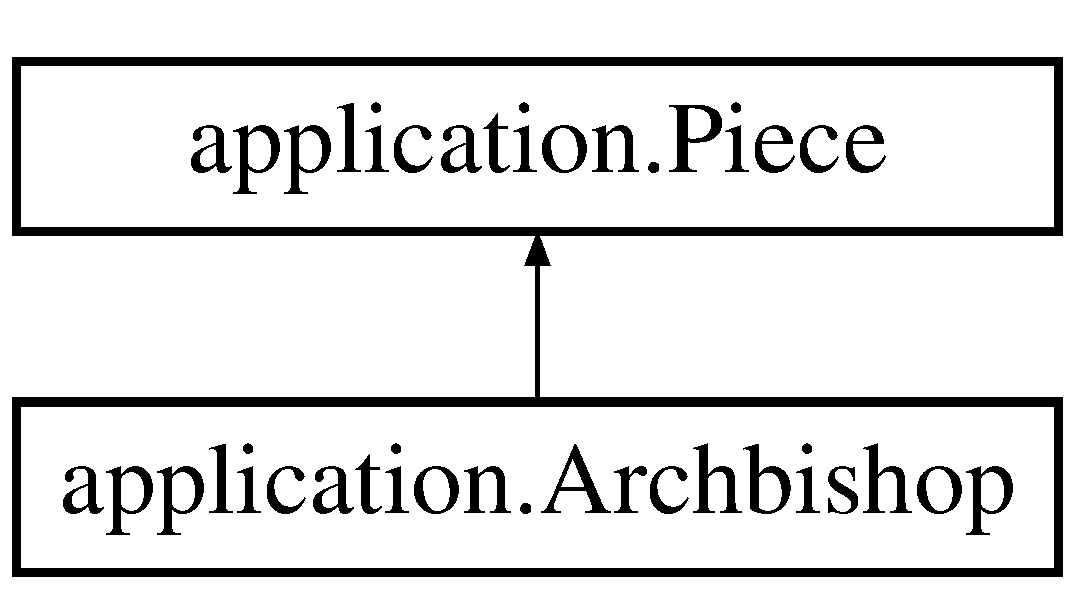
\includegraphics[height=2.000000cm]{classapplication_1_1_archbishop}
\end{center}
\end{figure}
\subsection*{Public Member Functions}
\begin{DoxyCompactItemize}
\item 
\hyperlink{classapplication_1_1_archbishop_a7089f574b3b187b5f9cdbc97985796cd}{Archbishop} (int x, int y, Game.\+O\+W\+N\+E\+R \hyperlink{classapplication_1_1_piece_a724f116bd99a66a6f6bcc8b7b35de131}{owner})
\begin{DoxyCompactList}\small\item\em Only constructor, simply sets internals to parameters and gathers some data from the \hyperlink{classapplication_1_1_map}{Map}. \end{DoxyCompactList}\item 
\hypertarget{classapplication_1_1_archbishop_a9cfee0021cca194c7ca87ad871a34a14}{void \hyperlink{classapplication_1_1_archbishop_a9cfee0021cca194c7ca87ad871a34a14}{get\+Moves} ()}\label{classapplication_1_1_archbishop_a9cfee0021cca194c7ca87ad871a34a14}

\begin{DoxyCompactList}\small\item\em Gets all available moves from the \hyperlink{classapplication_1_1_map}{Map} and stores them internally. \end{DoxyCompactList}\end{DoxyCompactItemize}
\subsection*{Additional Inherited Members}


\subsection{Detailed Description}
A \hyperlink{classapplication_1_1_piece}{Piece} object, moves in an \char`\"{}\+L\char`\"{} and in diagonals. 

\subsection{Constructor \& Destructor Documentation}
\hypertarget{classapplication_1_1_archbishop_a7089f574b3b187b5f9cdbc97985796cd}{\index{application\+::\+Archbishop@{application\+::\+Archbishop}!Archbishop@{Archbishop}}
\index{Archbishop@{Archbishop}!application\+::\+Archbishop@{application\+::\+Archbishop}}
\subsubsection[{Archbishop}]{\setlength{\rightskip}{0pt plus 5cm}application.\+Archbishop.\+Archbishop (
\begin{DoxyParamCaption}
\item[{int}]{x, }
\item[{int}]{y, }
\item[{Game.\+O\+W\+N\+E\+R}]{owner}
\end{DoxyParamCaption}
)\hspace{0.3cm}{\ttfamily [inline]}}}\label{classapplication_1_1_archbishop_a7089f574b3b187b5f9cdbc97985796cd}


Only constructor, simply sets internals to parameters and gathers some data from the \hyperlink{classapplication_1_1_map}{Map}. 


\begin{DoxyParams}{Parameters}
{\em x} & Integer specifying the x position \\
\hline
{\em y} & Integer specifying the y position \\
\hline
{\em owner} & O\+W\+N\+E\+R enumeration telling which player owns the \hyperlink{classapplication_1_1_piece}{Piece} \\
\hline
\end{DoxyParams}


The documentation for this class was generated from the following file\+:\begin{DoxyCompactItemize}
\item 
src/application/Archbishop.\+java\end{DoxyCompactItemize}

\hypertarget{classapplication_1_1_bishop}{\section{application.\+Bishop Class Reference}
\label{classapplication_1_1_bishop}\index{application.\+Bishop@{application.\+Bishop}}
}
Inheritance diagram for application.\+Bishop\+:\begin{figure}[H]
\begin{center}
\leavevmode
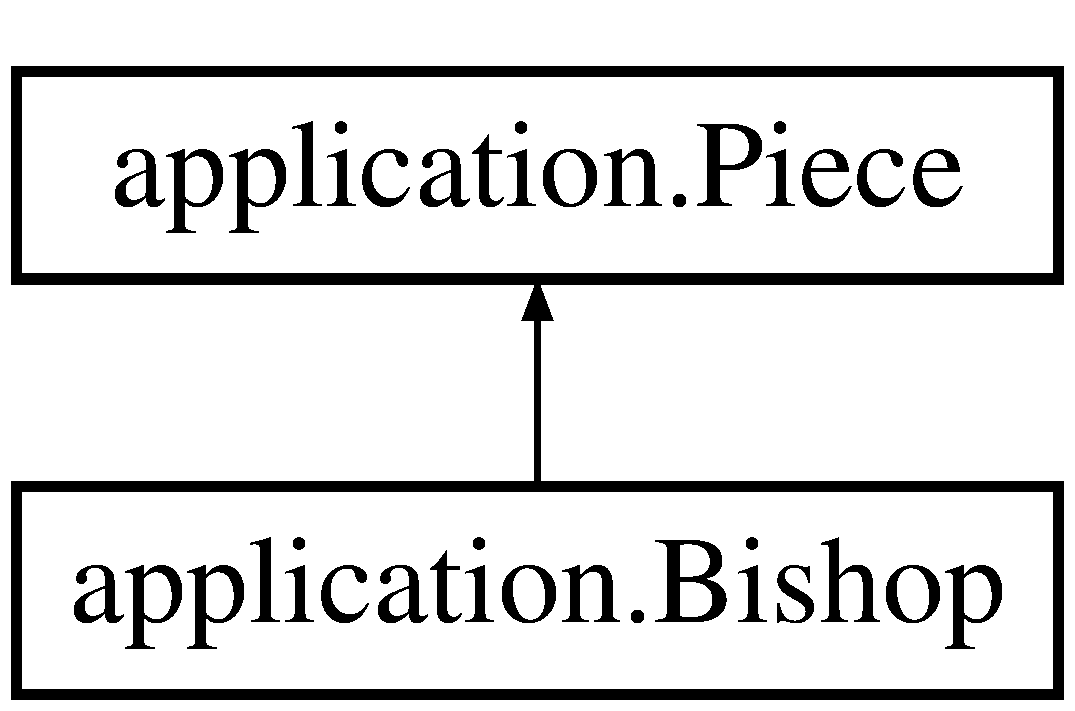
\includegraphics[height=2.000000cm]{classapplication_1_1_bishop}
\end{center}
\end{figure}
\subsection*{Public Member Functions}
\begin{DoxyCompactItemize}
\item 
\hypertarget{classapplication_1_1_bishop_a824e813916e5f1457225e6374c5a102b}{{\bfseries Bishop} (int x, int y, Game.\+O\+W\+N\+E\+R owner)}\label{classapplication_1_1_bishop_a824e813916e5f1457225e6374c5a102b}

\item 
\hypertarget{classapplication_1_1_bishop_a2b4021dea2118daf0647a19b610d83d9}{void {\bfseries get\+Moves} ()}\label{classapplication_1_1_bishop_a2b4021dea2118daf0647a19b610d83d9}

\end{DoxyCompactItemize}
\subsection*{Additional Inherited Members}


The documentation for this class was generated from the following file\+:\begin{DoxyCompactItemize}
\item 
src/application/Bishop.\+java\end{DoxyCompactItemize}

\hypertarget{classapplication_1_1_chancellor}{\section{application.\+Chancellor Class Reference}
\label{classapplication_1_1_chancellor}\index{application.\+Chancellor@{application.\+Chancellor}}
}


A \hyperlink{classapplication_1_1_piece}{Piece} object, moves in an \char`\"{}\+L\char`\"{} and across rows or columns.  


Inheritance diagram for application.\+Chancellor\+:\begin{figure}[H]
\begin{center}
\leavevmode
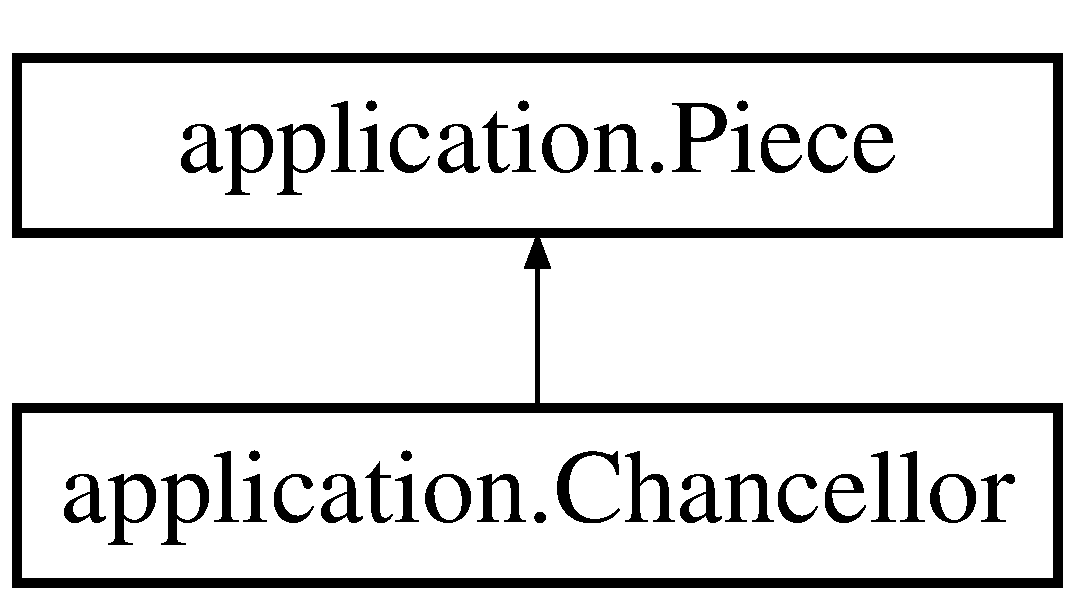
\includegraphics[height=2.000000cm]{classapplication_1_1_chancellor}
\end{center}
\end{figure}
\subsection*{Public Member Functions}
\begin{DoxyCompactItemize}
\item 
\hyperlink{classapplication_1_1_chancellor_a22e2dd42ff9699ffc8d430d5d3abb3e3}{Chancellor} (int x, int y, Game.\+O\+W\+N\+E\+R \hyperlink{classapplication_1_1_piece_a724f116bd99a66a6f6bcc8b7b35de131}{owner})
\begin{DoxyCompactList}\small\item\em Only constructor, simply sets internals to parameters and gathers some data from the \hyperlink{classapplication_1_1_map}{Map}. \end{DoxyCompactList}\item 
\hypertarget{classapplication_1_1_chancellor_a5fab8909007808c56e8ab511d738a543}{void \hyperlink{classapplication_1_1_chancellor_a5fab8909007808c56e8ab511d738a543}{get\+Moves} ()}\label{classapplication_1_1_chancellor_a5fab8909007808c56e8ab511d738a543}

\begin{DoxyCompactList}\small\item\em Gets all available moves from the \hyperlink{classapplication_1_1_map}{Map} and stores them internally. \end{DoxyCompactList}\end{DoxyCompactItemize}
\subsection*{Additional Inherited Members}


\subsection{Detailed Description}
A \hyperlink{classapplication_1_1_piece}{Piece} object, moves in an \char`\"{}\+L\char`\"{} and across rows or columns. 

\subsection{Constructor \& Destructor Documentation}
\hypertarget{classapplication_1_1_chancellor_a22e2dd42ff9699ffc8d430d5d3abb3e3}{\index{application\+::\+Chancellor@{application\+::\+Chancellor}!Chancellor@{Chancellor}}
\index{Chancellor@{Chancellor}!application\+::\+Chancellor@{application\+::\+Chancellor}}
\subsubsection[{Chancellor}]{\setlength{\rightskip}{0pt plus 5cm}application.\+Chancellor.\+Chancellor (
\begin{DoxyParamCaption}
\item[{int}]{x, }
\item[{int}]{y, }
\item[{Game.\+O\+W\+N\+E\+R}]{owner}
\end{DoxyParamCaption}
)\hspace{0.3cm}{\ttfamily [inline]}}}\label{classapplication_1_1_chancellor_a22e2dd42ff9699ffc8d430d5d3abb3e3}


Only constructor, simply sets internals to parameters and gathers some data from the \hyperlink{classapplication_1_1_map}{Map}. 


\begin{DoxyParams}{Parameters}
{\em x} & Integer specifying the x position \\
\hline
{\em y} & Integer specifying the y position \\
\hline
{\em owner} & O\+W\+N\+E\+R enumeration telling which player owns the \hyperlink{classapplication_1_1_piece}{Piece} \\
\hline
\end{DoxyParams}


The documentation for this class was generated from the following file\+:\begin{DoxyCompactItemize}
\item 
src/application/Chancellor.\+java\end{DoxyCompactItemize}

\hypertarget{classapplication_1_1_chess}{\section{application.\+Chess Class Reference}
\label{classapplication_1_1_chess}\index{application.\+Chess@{application.\+Chess}}
}


Main class, creates a \hyperlink{classapplication_1_1_game}{Game} and runs it.  


\subsection*{Static Public Member Functions}
\begin{DoxyCompactItemize}
\item 
static void \hyperlink{classapplication_1_1_chess_aa724f30b1b436386ea596dcee0680aa6}{main} (String\mbox{[}$\,$\mbox{]} args)
\begin{DoxyCompactList}\small\item\em Main function, creates \hyperlink{classapplication_1_1_game}{Game} and calls run on it. \end{DoxyCompactList}\end{DoxyCompactItemize}


\subsection{Detailed Description}
Main class, creates a \hyperlink{classapplication_1_1_game}{Game} and runs it. 

\subsection{Member Function Documentation}
\hypertarget{classapplication_1_1_chess_aa724f30b1b436386ea596dcee0680aa6}{\index{application\+::\+Chess@{application\+::\+Chess}!main@{main}}
\index{main@{main}!application\+::\+Chess@{application\+::\+Chess}}
\subsubsection[{main}]{\setlength{\rightskip}{0pt plus 5cm}static void application.\+Chess.\+main (
\begin{DoxyParamCaption}
\item[{String\mbox{[}$\,$\mbox{]}}]{args}
\end{DoxyParamCaption}
)\hspace{0.3cm}{\ttfamily [inline]}, {\ttfamily [static]}}}\label{classapplication_1_1_chess_aa724f30b1b436386ea596dcee0680aa6}


Main function, creates \hyperlink{classapplication_1_1_game}{Game} and calls run on it. 


\begin{DoxyParams}{Parameters}
{\em args} & No effect on program \\
\hline
\end{DoxyParams}


The documentation for this class was generated from the following file\+:\begin{DoxyCompactItemize}
\item 
src/application/Chess.\+java\end{DoxyCompactItemize}

\hypertarget{classapplication_1_1_game}{\section{application.\+Game Class Reference}
\label{classapplication_1_1_game}\index{application.\+Game@{application.\+Game}}
}
\subsection*{Classes}
\begin{DoxyCompactItemize}
\item 
enum {\bfseries O\+W\+N\+E\+R}
\item 
enum {\bfseries S\+T\+A\+T\+E}
\end{DoxyCompactItemize}
\subsection*{Public Member Functions}
\begin{DoxyCompactItemize}
\item 
\hypertarget{classapplication_1_1_game_a35f63ec92d69c27a46171e54477a4783}{void {\bfseries run} ()}\label{classapplication_1_1_game_a35f63ec92d69c27a46171e54477a4783}

\end{DoxyCompactItemize}
\subsection*{Static Public Attributes}
\begin{DoxyCompactItemize}
\item 
\hypertarget{classapplication_1_1_game_a10619b2e871df9e6de819b032cbe1a4d}{static \hyperlink{classapplication_1_1_map}{Map} {\bfseries map}}\label{classapplication_1_1_game_a10619b2e871df9e6de819b032cbe1a4d}

\item 
\hypertarget{classapplication_1_1_game_a08866c12070f0ef544abd8b9f1b6b0e5}{static \hyperlink{classapplication_1_1_player}{Player} {\bfseries player\+One}}\label{classapplication_1_1_game_a08866c12070f0ef544abd8b9f1b6b0e5}

\item 
\hypertarget{classapplication_1_1_game_a31fcad6171766180e0eef67f71253532}{static \hyperlink{classapplication_1_1_player}{Player} {\bfseries player\+Two}}\label{classapplication_1_1_game_a31fcad6171766180e0eef67f71253532}

\item 
\hypertarget{classapplication_1_1_game_adb74b89e0a6424ebcd5c5c13bb569e0c}{static S\+T\+A\+T\+E {\bfseries state}}\label{classapplication_1_1_game_adb74b89e0a6424ebcd5c5c13bb569e0c}

\item 
\hypertarget{classapplication_1_1_game_ad90cfa46ef32022357de71db5f1f7184}{static O\+W\+N\+E\+R {\bfseries turn}}\label{classapplication_1_1_game_ad90cfa46ef32022357de71db5f1f7184}

\end{DoxyCompactItemize}


The documentation for this class was generated from the following file\+:\begin{DoxyCompactItemize}
\item 
src/application/Game.\+java\end{DoxyCompactItemize}

\hypertarget{classapplication_1_1_king}{\section{application.\+King Class Reference}
\label{classapplication_1_1_king}\index{application.\+King@{application.\+King}}
}
Inheritance diagram for application.\+King\+:\begin{figure}[H]
\begin{center}
\leavevmode
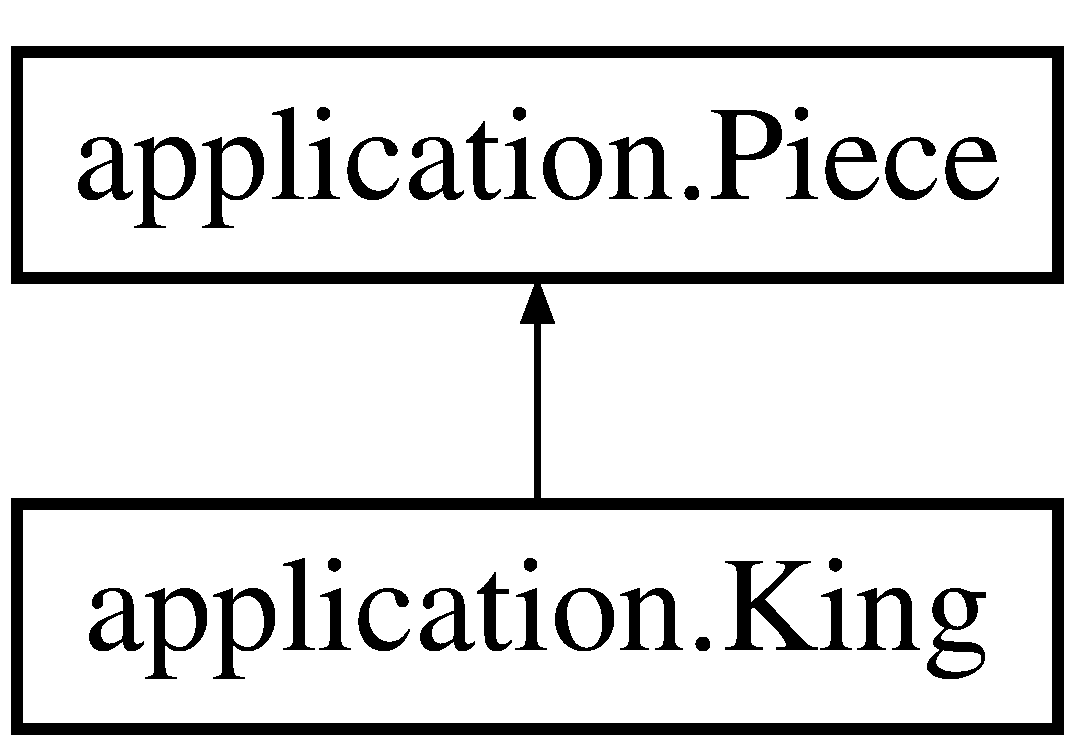
\includegraphics[height=2.000000cm]{classapplication_1_1_king}
\end{center}
\end{figure}
\subsection*{Public Member Functions}
\begin{DoxyCompactItemize}
\item 
\hypertarget{classapplication_1_1_king_aaf752b3e54e7ef1c51263c2493212a5f}{{\bfseries King} (int x, int y, Game.\+O\+W\+N\+E\+R owner)}\label{classapplication_1_1_king_aaf752b3e54e7ef1c51263c2493212a5f}

\item 
\hypertarget{classapplication_1_1_king_adb6361fe24a37fbe385e8e3aa626163e}{void {\bfseries get\+Moves} ()}\label{classapplication_1_1_king_adb6361fe24a37fbe385e8e3aa626163e}

\end{DoxyCompactItemize}
\subsection*{Additional Inherited Members}


The documentation for this class was generated from the following file\+:\begin{DoxyCompactItemize}
\item 
src/application/King.\+java\end{DoxyCompactItemize}

\hypertarget{classapplication_1_1_knight}{\section{application.\+Knight Class Reference}
\label{classapplication_1_1_knight}\index{application.\+Knight@{application.\+Knight}}
}


A \hyperlink{classapplication_1_1_piece}{Piece} object, moves in an \char`\"{}\+L\char`\"{} and can jump pieces.  


Inheritance diagram for application.\+Knight\+:\begin{figure}[H]
\begin{center}
\leavevmode
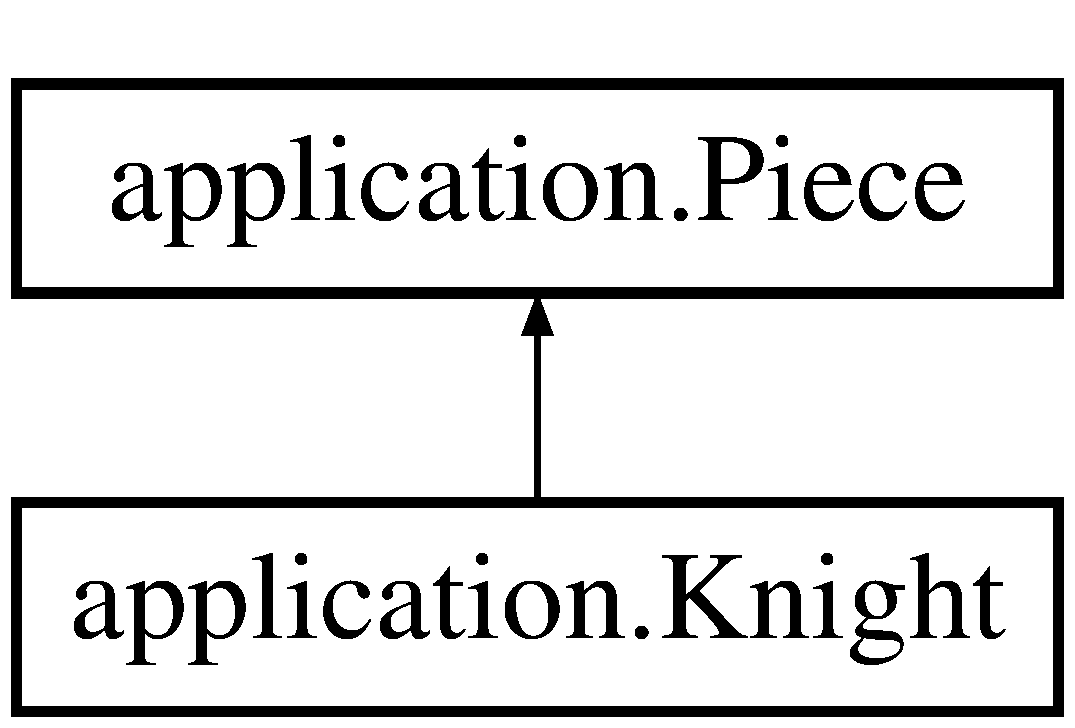
\includegraphics[height=2.000000cm]{classapplication_1_1_knight}
\end{center}
\end{figure}
\subsection*{Public Member Functions}
\begin{DoxyCompactItemize}
\item 
\hyperlink{classapplication_1_1_knight_a514487094841cbb827eea58b780f488e}{Knight} (int x, int y, Game.\+O\+W\+N\+E\+R \hyperlink{classapplication_1_1_piece_a724f116bd99a66a6f6bcc8b7b35de131}{owner})
\begin{DoxyCompactList}\small\item\em Only constructor, simply sets internals to parameters and gathers some data from the \hyperlink{classapplication_1_1_map}{Map}. \end{DoxyCompactList}\item 
\hypertarget{classapplication_1_1_knight_adf3b8759d81165000cf35274ba4e36b2}{void \hyperlink{classapplication_1_1_knight_adf3b8759d81165000cf35274ba4e36b2}{get\+Moves} ()}\label{classapplication_1_1_knight_adf3b8759d81165000cf35274ba4e36b2}

\begin{DoxyCompactList}\small\item\em Gets all available moves from the \hyperlink{classapplication_1_1_map}{Map} and stores them internally. \end{DoxyCompactList}\end{DoxyCompactItemize}
\subsection*{Additional Inherited Members}


\subsection{Detailed Description}
A \hyperlink{classapplication_1_1_piece}{Piece} object, moves in an \char`\"{}\+L\char`\"{} and can jump pieces. 

\subsection{Constructor \& Destructor Documentation}
\hypertarget{classapplication_1_1_knight_a514487094841cbb827eea58b780f488e}{\index{application\+::\+Knight@{application\+::\+Knight}!Knight@{Knight}}
\index{Knight@{Knight}!application\+::\+Knight@{application\+::\+Knight}}
\subsubsection[{Knight}]{\setlength{\rightskip}{0pt plus 5cm}application.\+Knight.\+Knight (
\begin{DoxyParamCaption}
\item[{int}]{x, }
\item[{int}]{y, }
\item[{Game.\+O\+W\+N\+E\+R}]{owner}
\end{DoxyParamCaption}
)\hspace{0.3cm}{\ttfamily [inline]}}}\label{classapplication_1_1_knight_a514487094841cbb827eea58b780f488e}


Only constructor, simply sets internals to parameters and gathers some data from the \hyperlink{classapplication_1_1_map}{Map}. 


\begin{DoxyParams}{Parameters}
{\em x} & Integer specifying the x position \\
\hline
{\em y} & Integer specifying the y position \\
\hline
{\em owner} & O\+W\+N\+E\+R enumeration telling which player owns the \hyperlink{classapplication_1_1_piece}{Piece} \\
\hline
\end{DoxyParams}


The documentation for this class was generated from the following file\+:\begin{DoxyCompactItemize}
\item 
src/application/Knight.\+java\end{DoxyCompactItemize}

\hypertarget{classapplication_1_1_map}{\section{application.\+Map Class Reference}
\label{classapplication_1_1_map}\index{application.\+Map@{application.\+Map}}
}
\subsection*{Public Member Functions}
\begin{DoxyCompactItemize}
\item 
\hypertarget{classapplication_1_1_map_a405c4fa754f25e33bd8eafee061d1c5d}{void {\bfseries update} ()}\label{classapplication_1_1_map_a405c4fa754f25e33bd8eafee061d1c5d}

\item 
\hypertarget{classapplication_1_1_map_a0b9639952785a325be6f0251e4120658}{void {\bfseries draw} ()}\label{classapplication_1_1_map_a0b9639952785a325be6f0251e4120658}

\item 
\hypertarget{classapplication_1_1_map_a0bdc2326a0f637cc37877f480546e8cd}{Vector$<$ \hyperlink{classapplication_1_1_pair}{Pair} $>$ {\bfseries get\+Row\+Positions\+At} (int x, int y, Game.\+O\+W\+N\+E\+R owner)}\label{classapplication_1_1_map_a0bdc2326a0f637cc37877f480546e8cd}

\item 
\hypertarget{classapplication_1_1_map_a7236d3894ef2460f49341c63ca24d30a}{Vector$<$ \hyperlink{classapplication_1_1_pair}{Pair} $>$ {\bfseries get\+Column\+Positions\+At} (int x, int y, Game.\+O\+W\+N\+E\+R owner)}\label{classapplication_1_1_map_a7236d3894ef2460f49341c63ca24d30a}

\item 
\hypertarget{classapplication_1_1_map_a57789d28a30b28e06bc2f34bfc0ea114}{Vector$<$ \hyperlink{classapplication_1_1_pair}{Pair} $>$ {\bfseries get\+Diagonal\+B\+Lto\+T\+R} (int x, int y, Game.\+O\+W\+N\+E\+R owner)}\label{classapplication_1_1_map_a57789d28a30b28e06bc2f34bfc0ea114}

\item 
\hypertarget{classapplication_1_1_map_af3f89ab9eda95d77a1ea1f135ec69b0a}{Vector$<$ \hyperlink{classapplication_1_1_pair}{Pair} $>$ {\bfseries get\+Diagonal\+T\+Lto\+B\+R} (int x, int y, Game.\+O\+W\+N\+E\+R owner)}\label{classapplication_1_1_map_af3f89ab9eda95d77a1ea1f135ec69b0a}

\item 
\hypertarget{classapplication_1_1_map_a2cbd93ac3f3085fff563bd26a45524ba}{boolean {\bfseries in\+Bounds} (int x, int y)}\label{classapplication_1_1_map_a2cbd93ac3f3085fff563bd26a45524ba}

\item 
\hypertarget{classapplication_1_1_map_a4c8ecfb3c342531fcf2e82b9951dacd9}{boolean {\bfseries check\+Tile\+Occupied} (int x, int y)}\label{classapplication_1_1_map_a4c8ecfb3c342531fcf2e82b9951dacd9}

\item 
\hypertarget{classapplication_1_1_map_ace2bcd71a180c9abcc48299dbded34f8}{boolean {\bfseries check\+Tile\+Enemy} (int x, int y, Game.\+O\+W\+N\+E\+R owner)}\label{classapplication_1_1_map_ace2bcd71a180c9abcc48299dbded34f8}

\item 
\hypertarget{classapplication_1_1_map_acf9ab16c56c49259ce5435e708db81d3}{int {\bfseries get\+Width} ()}\label{classapplication_1_1_map_acf9ab16c56c49259ce5435e708db81d3}

\item 
\hypertarget{classapplication_1_1_map_a937a0d16608ab0f866484f50cf3e2756}{int {\bfseries get\+Height} ()}\label{classapplication_1_1_map_a937a0d16608ab0f866484f50cf3e2756}

\item 
\hypertarget{classapplication_1_1_map_a1f0155540d45815c84b1f1fef5c02b78}{int {\bfseries get\+Tile\+Width} ()}\label{classapplication_1_1_map_a1f0155540d45815c84b1f1fef5c02b78}

\item 
\hypertarget{classapplication_1_1_map_aed96fe881a45be9f60937b28228e5690}{int {\bfseries get\+Tile\+Height} ()}\label{classapplication_1_1_map_aed96fe881a45be9f60937b28228e5690}

\item 
\hypertarget{classapplication_1_1_map_abc7ffbed0a366b2e703b1ea3757d0d6a}{void {\bfseries set\+Tile\+Owner} (int x, int y, Game.\+O\+W\+N\+E\+R owner)}\label{classapplication_1_1_map_abc7ffbed0a366b2e703b1ea3757d0d6a}

\end{DoxyCompactItemize}


The documentation for this class was generated from the following file\+:\begin{DoxyCompactItemize}
\item 
src/application/Map.\+java\end{DoxyCompactItemize}

\hypertarget{classapplication_1_1_map_tile}{\section{application.\+Map\+Tile Class Reference}
\label{classapplication_1_1_map_tile}\index{application.\+Map\+Tile@{application.\+Map\+Tile}}
}


A simple object which makes up the \hyperlink{classapplication_1_1_map}{Map}, and stores who owns it.  


\subsection*{Public Member Functions}
\begin{DoxyCompactItemize}
\item 
\hypertarget{classapplication_1_1_map_tile_a05f16549a120e72840b79f668af59c4a}{\hyperlink{classapplication_1_1_map_tile_a05f16549a120e72840b79f668af59c4a}{Map\+Tile} ()}\label{classapplication_1_1_map_tile_a05f16549a120e72840b79f668af59c4a}

\begin{DoxyCompactList}\small\item\em Default constructor, sets owner to N\+O\+N\+E. \end{DoxyCompactList}\end{DoxyCompactItemize}
\subsection*{Public Attributes}
\begin{DoxyCompactItemize}
\item 
\hypertarget{classapplication_1_1_map_tile_a720b9fc0678031d85d5e676a0a0cb49f}{Game.\+O\+W\+N\+E\+R \hyperlink{classapplication_1_1_map_tile_a720b9fc0678031d85d5e676a0a0cb49f}{owner}}\label{classapplication_1_1_map_tile_a720b9fc0678031d85d5e676a0a0cb49f}

\begin{DoxyCompactList}\small\item\em O\+W\+N\+E\+R enumeration of who owns the tile. \end{DoxyCompactList}\end{DoxyCompactItemize}


\subsection{Detailed Description}
A simple object which makes up the \hyperlink{classapplication_1_1_map}{Map}, and stores who owns it. 

The documentation for this class was generated from the following file\+:\begin{DoxyCompactItemize}
\item 
src/application/Map\+Tile.\+java\end{DoxyCompactItemize}

\hypertarget{classapplication_1_1_pair}{\section{application.\+Pair Class Reference}
\label{classapplication_1_1_pair}\index{application.\+Pair@{application.\+Pair}}
}


Custom pair object, simply holds and x and y integer.  


\subsection*{Public Attributes}
\begin{DoxyCompactItemize}
\item 
\hypertarget{classapplication_1_1_pair_af1c4cefc5c3a56acf3be3028d3be44bd}{int \hyperlink{classapplication_1_1_pair_af1c4cefc5c3a56acf3be3028d3be44bd}{x}}\label{classapplication_1_1_pair_af1c4cefc5c3a56acf3be3028d3be44bd}

\begin{DoxyCompactList}\small\item\em x component, an integer \end{DoxyCompactList}\item 
\hypertarget{classapplication_1_1_pair_a1d64330494663f25fe62a8cea5f30dc1}{int \hyperlink{classapplication_1_1_pair_a1d64330494663f25fe62a8cea5f30dc1}{y}}\label{classapplication_1_1_pair_a1d64330494663f25fe62a8cea5f30dc1}

\begin{DoxyCompactList}\small\item\em y component, an integer \end{DoxyCompactList}\end{DoxyCompactItemize}


\subsection{Detailed Description}
Custom pair object, simply holds and x and y integer. 

The documentation for this class was generated from the following file\+:\begin{DoxyCompactItemize}
\item 
src/application/Pair.\+java\end{DoxyCompactItemize}

\hypertarget{classapplication_1_1_pawn}{\section{application.\+Pawn Class Reference}
\label{classapplication_1_1_pawn}\index{application.\+Pawn@{application.\+Pawn}}
}
Inheritance diagram for application.\+Pawn\+:\begin{figure}[H]
\begin{center}
\leavevmode
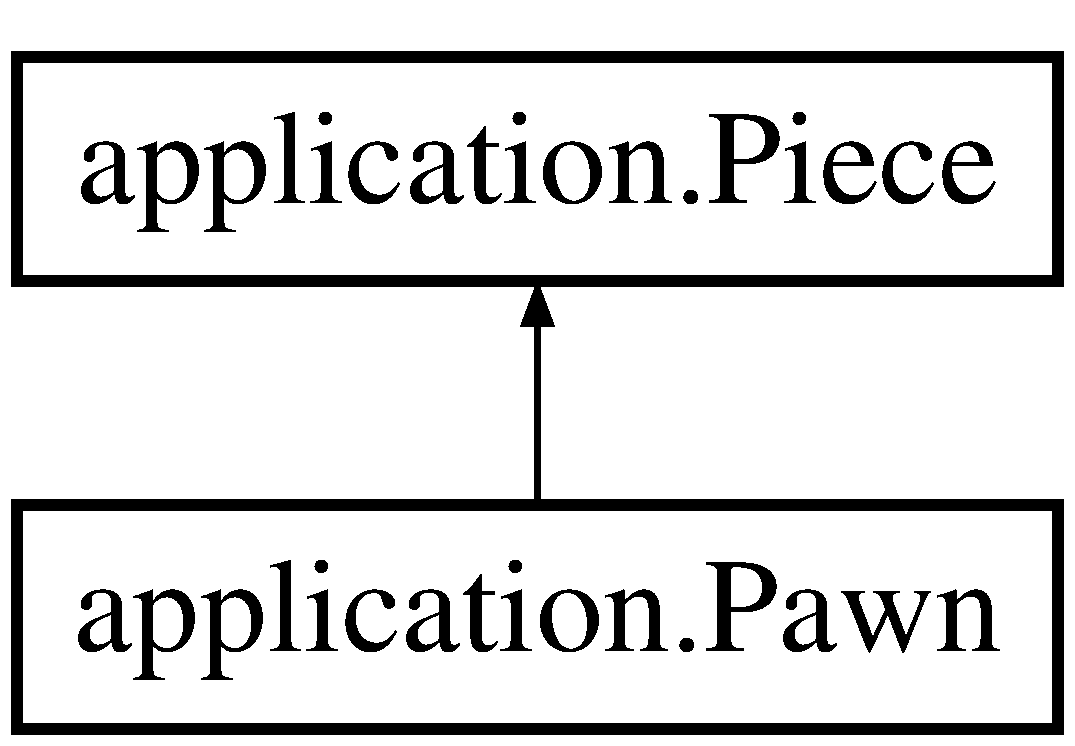
\includegraphics[height=2.000000cm]{classapplication_1_1_pawn}
\end{center}
\end{figure}
\subsection*{Public Member Functions}
\begin{DoxyCompactItemize}
\item 
\hypertarget{classapplication_1_1_pawn_aa4d6c3a524dabd13c17a220bfd5db423}{{\bfseries Pawn} (int x, int y, Game.\+O\+W\+N\+E\+R owner)}\label{classapplication_1_1_pawn_aa4d6c3a524dabd13c17a220bfd5db423}

\item 
\hypertarget{classapplication_1_1_pawn_a0a43e16b2e2d80001617aeb0cd0ad440}{void {\bfseries get\+Moves} ()}\label{classapplication_1_1_pawn_a0a43e16b2e2d80001617aeb0cd0ad440}

\end{DoxyCompactItemize}
\subsection*{Additional Inherited Members}


The documentation for this class was generated from the following file\+:\begin{DoxyCompactItemize}
\item 
src/application/Pawn.\+java\end{DoxyCompactItemize}

\hypertarget{classapplication_1_1_piece}{\section{application.\+Piece Class Reference}
\label{classapplication_1_1_piece}\index{application.\+Piece@{application.\+Piece}}
}
Inheritance diagram for application.\+Piece\+:\begin{figure}[H]
\begin{center}
\leavevmode
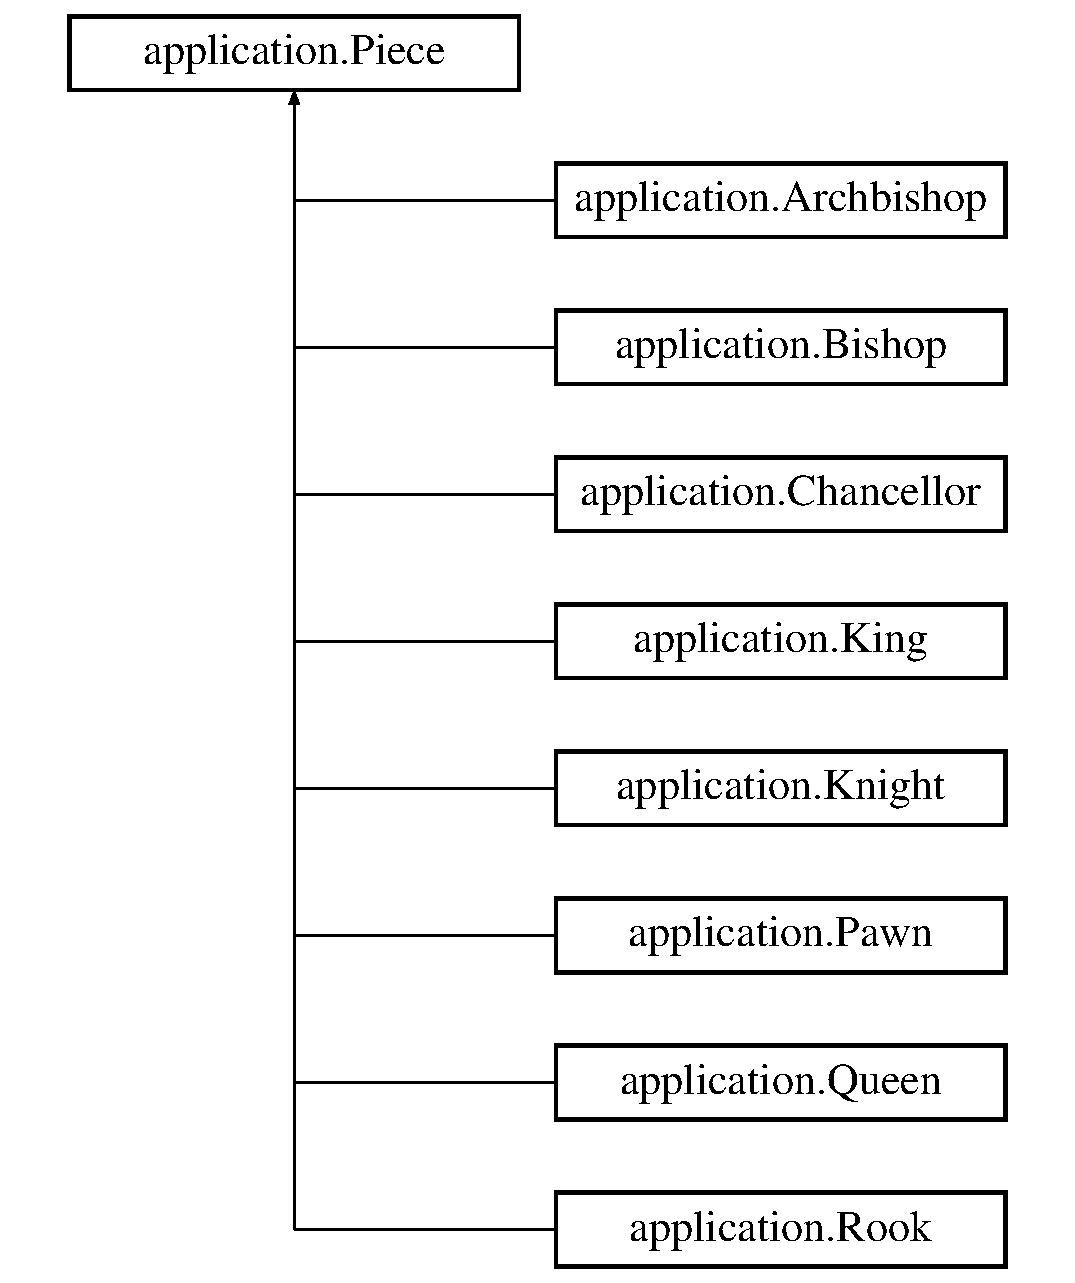
\includegraphics[height=1.517615cm]{classapplication_1_1_piece}
\end{center}
\end{figure}
\subsection*{Public Member Functions}
\begin{DoxyCompactItemize}
\item 
\hypertarget{classapplication_1_1_piece_a7845605267af2d616efc66af07d175ea}{{\bfseries Piece} (int x, int y, Game.\+O\+W\+N\+E\+R owner)}\label{classapplication_1_1_piece_a7845605267af2d616efc66af07d175ea}

\item 
\hypertarget{classapplication_1_1_piece_ae4bdd8cfc85f889c8d7dc840a137cd65}{void {\bfseries draw} ()}\label{classapplication_1_1_piece_ae4bdd8cfc85f889c8d7dc840a137cd65}

\item 
\hypertarget{classapplication_1_1_piece_acca039f617b0bf259eb1e1d00fbf4cda}{void {\bfseries get\+Moves} ()}\label{classapplication_1_1_piece_acca039f617b0bf259eb1e1d00fbf4cda}

\item 
\hypertarget{classapplication_1_1_piece_ac91b28148a2b0e38edeba7a42501d99f}{void {\bfseries move\+To} (int x, int y)}\label{classapplication_1_1_piece_ac91b28148a2b0e38edeba7a42501d99f}

\item 
\hypertarget{classapplication_1_1_piece_a2e58a2e63e94dd3de909e2fd55a7b819}{int {\bfseries get\+X} ()}\label{classapplication_1_1_piece_a2e58a2e63e94dd3de909e2fd55a7b819}

\item 
\hypertarget{classapplication_1_1_piece_a360e6e106c1254e4b86e69143ca0ce72}{int {\bfseries get\+Y} ()}\label{classapplication_1_1_piece_a360e6e106c1254e4b86e69143ca0ce72}

\end{DoxyCompactItemize}
\subsection*{Protected Member Functions}
\begin{DoxyCompactItemize}
\item 
\hypertarget{classapplication_1_1_piece_a70d0ea8dfe2d8ebaf1af52f3468cf972}{void {\bfseries check\+Moves} ()}\label{classapplication_1_1_piece_a70d0ea8dfe2d8ebaf1af52f3468cf972}

\end{DoxyCompactItemize}
\subsection*{Protected Attributes}
\begin{DoxyCompactItemize}
\item 
\hypertarget{classapplication_1_1_piece_af7a78ee6a0bbbee54b0bf385ab3eda43}{int {\bfseries x\+Pos}}\label{classapplication_1_1_piece_af7a78ee6a0bbbee54b0bf385ab3eda43}

\item 
\hypertarget{classapplication_1_1_piece_a11da2d0872e6553217daa56a851c7740}{int {\bfseries y\+Pos}}\label{classapplication_1_1_piece_a11da2d0872e6553217daa56a851c7740}

\item 
\hypertarget{classapplication_1_1_piece_a8885ca50301c6e85d333f397ad106a6b}{int {\bfseries width}}\label{classapplication_1_1_piece_a8885ca50301c6e85d333f397ad106a6b}

\item 
\hypertarget{classapplication_1_1_piece_af7f74a095a34bf775cc6b44e5ea1dcbe}{int {\bfseries height}}\label{classapplication_1_1_piece_af7f74a095a34bf775cc6b44e5ea1dcbe}

\item 
\hypertarget{classapplication_1_1_piece_a423e3460410ce4199060a42812c79463}{Buffered\+Image {\bfseries img}}\label{classapplication_1_1_piece_a423e3460410ce4199060a42812c79463}

\item 
\hypertarget{classapplication_1_1_piece_a9e704a1ebc750f4a5f1c640f1cc927f4}{Vector$<$ \hyperlink{classapplication_1_1_pair}{Pair} $>$ {\bfseries moves}}\label{classapplication_1_1_piece_a9e704a1ebc750f4a5f1c640f1cc927f4}

\item 
\hypertarget{classapplication_1_1_piece_a724f116bd99a66a6f6bcc8b7b35de131}{Game.\+O\+W\+N\+E\+R {\bfseries owner}}\label{classapplication_1_1_piece_a724f116bd99a66a6f6bcc8b7b35de131}

\item 
\hypertarget{classapplication_1_1_piece_a8610c3152130255360304aabb534e7cb}{boolean {\bfseries first\+Move}}\label{classapplication_1_1_piece_a8610c3152130255360304aabb534e7cb}

\end{DoxyCompactItemize}


The documentation for this class was generated from the following file\+:\begin{DoxyCompactItemize}
\item 
src/application/Piece.\+java\end{DoxyCompactItemize}

\hypertarget{classapplication_1_1_player}{\section{application.\+Player Class Reference}
\label{classapplication_1_1_player}\index{application.\+Player@{application.\+Player}}
}


This keeps tracks of all Pieces, along with drawing and selection.  


\subsection*{Public Member Functions}
\begin{DoxyCompactItemize}
\item 
\hyperlink{classapplication_1_1_player_a14ac1e2c788fb22e7e5be4e5e6bc1847}{Player} (Game.\+O\+W\+N\+E\+R player\+Num)
\begin{DoxyCompactList}\small\item\em Only constructor, adds pieces to board. \end{DoxyCompactList}\item 
\hypertarget{classapplication_1_1_player_a0fd6b813c9a0ab1e9844d0c13d709a44}{void \hyperlink{classapplication_1_1_player_a0fd6b813c9a0ab1e9844d0c13d709a44}{draw\+Moves} ()}\label{classapplication_1_1_player_a0fd6b813c9a0ab1e9844d0c13d709a44}

\begin{DoxyCompactList}\small\item\em Draw possible moves of selected piece. \end{DoxyCompactList}\item 
\hypertarget{classapplication_1_1_player_ad598f6c101732c33ced27c1ec23b7080}{void \hyperlink{classapplication_1_1_player_ad598f6c101732c33ced27c1ec23b7080}{draw\+Pieces} ()}\label{classapplication_1_1_player_ad598f6c101732c33ced27c1ec23b7080}

\begin{DoxyCompactList}\small\item\em Draw pieces on board, calls draw function of each piece. \end{DoxyCompactList}\item 
void \hyperlink{classapplication_1_1_player_abc096ccded0197ea0a5a87e09b55507e}{select} (int x, int y)
\begin{DoxyCompactList}\small\item\em Handle action of clicking at (x,y), depending on \hyperlink{classapplication_1_1_game}{Game} state and turn. \end{DoxyCompactList}\item 
void \hyperlink{classapplication_1_1_player_a82638976ae19fce3c6e03b589938abaa}{kill\+At} (int x, int y)
\begin{DoxyCompactList}\small\item\em Removes \hyperlink{classapplication_1_1_piece}{Piece} at (x,y) \end{DoxyCompactList}\end{DoxyCompactItemize}
\subsection*{Public Attributes}
\begin{DoxyCompactItemize}
\item 
\hypertarget{classapplication_1_1_player_ade2a529ac843368e351446cde7e6f76b}{Vector$<$ \hyperlink{classapplication_1_1_piece}{Piece} $>$ \hyperlink{classapplication_1_1_player_ade2a529ac843368e351446cde7e6f76b}{pieces}}\label{classapplication_1_1_player_ade2a529ac843368e351446cde7e6f76b}

\begin{DoxyCompactList}\small\item\em Vector which holds what Pieces the player owns. \end{DoxyCompactList}\end{DoxyCompactItemize}


\subsection{Detailed Description}
This keeps tracks of all Pieces, along with drawing and selection. 

\subsection{Constructor \& Destructor Documentation}
\hypertarget{classapplication_1_1_player_a14ac1e2c788fb22e7e5be4e5e6bc1847}{\index{application\+::\+Player@{application\+::\+Player}!Player@{Player}}
\index{Player@{Player}!application\+::\+Player@{application\+::\+Player}}
\subsubsection[{Player}]{\setlength{\rightskip}{0pt plus 5cm}application.\+Player.\+Player (
\begin{DoxyParamCaption}
\item[{Game.\+O\+W\+N\+E\+R}]{player\+Num}
\end{DoxyParamCaption}
)\hspace{0.3cm}{\ttfamily [inline]}}}\label{classapplication_1_1_player_a14ac1e2c788fb22e7e5be4e5e6bc1847}


Only constructor, adds pieces to board. 


\begin{DoxyParams}{Parameters}
{\em player\+Num} & Which player this is, to set ownership of pieces \\
\hline
\end{DoxyParams}


\subsection{Member Function Documentation}
\hypertarget{classapplication_1_1_player_a82638976ae19fce3c6e03b589938abaa}{\index{application\+::\+Player@{application\+::\+Player}!kill\+At@{kill\+At}}
\index{kill\+At@{kill\+At}!application\+::\+Player@{application\+::\+Player}}
\subsubsection[{kill\+At}]{\setlength{\rightskip}{0pt plus 5cm}void application.\+Player.\+kill\+At (
\begin{DoxyParamCaption}
\item[{int}]{x, }
\item[{int}]{y}
\end{DoxyParamCaption}
)\hspace{0.3cm}{\ttfamily [inline]}}}\label{classapplication_1_1_player_a82638976ae19fce3c6e03b589938abaa}


Removes \hyperlink{classapplication_1_1_piece}{Piece} at (x,y) 


\begin{DoxyParams}{Parameters}
{\em x} & x-\/coordinate to remove \hyperlink{classapplication_1_1_piece}{Piece} from \\
\hline
{\em y} & y-\/coordinate to remove \hyperlink{classapplication_1_1_piece}{Piece} from \\
\hline
\end{DoxyParams}
\hypertarget{classapplication_1_1_player_abc096ccded0197ea0a5a87e09b55507e}{\index{application\+::\+Player@{application\+::\+Player}!select@{select}}
\index{select@{select}!application\+::\+Player@{application\+::\+Player}}
\subsubsection[{select}]{\setlength{\rightskip}{0pt plus 5cm}void application.\+Player.\+select (
\begin{DoxyParamCaption}
\item[{int}]{x, }
\item[{int}]{y}
\end{DoxyParamCaption}
)\hspace{0.3cm}{\ttfamily [inline]}}}\label{classapplication_1_1_player_abc096ccded0197ea0a5a87e09b55507e}


Handle action of clicking at (x,y), depending on \hyperlink{classapplication_1_1_game}{Game} state and turn. 


\begin{DoxyParams}{Parameters}
{\em x} & x-\/coordinate on \hyperlink{classapplication_1_1_map}{Map} \\
\hline
{\em y} & y-\/coordinate on \hyperlink{classapplication_1_1_map}{Map} \\
\hline
\end{DoxyParams}


The documentation for this class was generated from the following file\+:\begin{DoxyCompactItemize}
\item 
src/application/Player.\+java\end{DoxyCompactItemize}

\hypertarget{classapplication_1_1_queen}{\section{application.\+Queen Class Reference}
\label{classapplication_1_1_queen}\index{application.\+Queen@{application.\+Queen}}
}
Inheritance diagram for application.\+Queen\+:\begin{figure}[H]
\begin{center}
\leavevmode
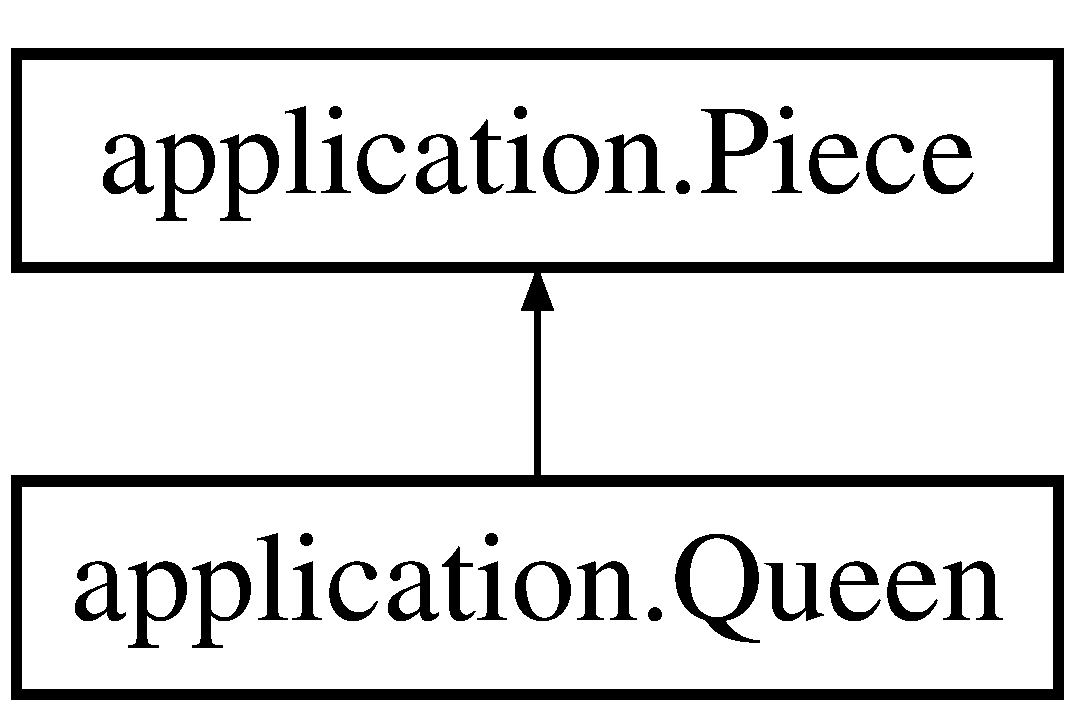
\includegraphics[height=2.000000cm]{classapplication_1_1_queen}
\end{center}
\end{figure}
\subsection*{Public Member Functions}
\begin{DoxyCompactItemize}
\item 
\hypertarget{classapplication_1_1_queen_a72921fc90666a1931a1e058d0ab63e85}{{\bfseries Queen} (int x, int y, Game.\+O\+W\+N\+E\+R owner)}\label{classapplication_1_1_queen_a72921fc90666a1931a1e058d0ab63e85}

\item 
\hypertarget{classapplication_1_1_queen_ab020c2fde4eeb0f6d5e6020434d90b1f}{void {\bfseries get\+Moves} ()}\label{classapplication_1_1_queen_ab020c2fde4eeb0f6d5e6020434d90b1f}

\end{DoxyCompactItemize}
\subsection*{Additional Inherited Members}


The documentation for this class was generated from the following file\+:\begin{DoxyCompactItemize}
\item 
src/application/Queen.\+java\end{DoxyCompactItemize}

\hypertarget{classapplication_1_1_rook}{\section{application.\+Rook Class Reference}
\label{classapplication_1_1_rook}\index{application.\+Rook@{application.\+Rook}}
}


A \hyperlink{classapplication_1_1_piece}{Piece} object, moves across rows and columns.  


Inheritance diagram for application.\+Rook\+:\begin{figure}[H]
\begin{center}
\leavevmode
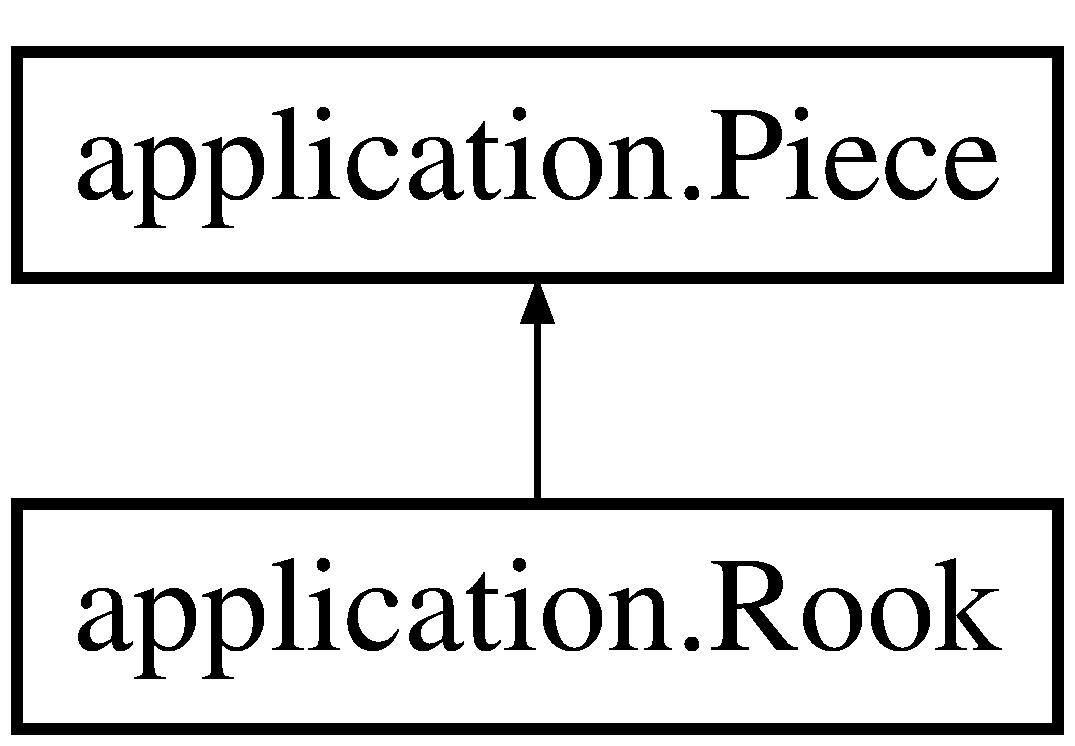
\includegraphics[height=2.000000cm]{classapplication_1_1_rook}
\end{center}
\end{figure}
\subsection*{Public Member Functions}
\begin{DoxyCompactItemize}
\item 
\hyperlink{classapplication_1_1_rook_a748877f5e1bfca7a705a19b1832c5629}{Rook} (int x, int y, Game.\+O\+W\+N\+E\+R \hyperlink{classapplication_1_1_piece_a724f116bd99a66a6f6bcc8b7b35de131}{owner})
\begin{DoxyCompactList}\small\item\em Only constructor, simply sets internals to parameters and gathers some data from the \hyperlink{classapplication_1_1_map}{Map}. \end{DoxyCompactList}\item 
\hypertarget{classapplication_1_1_rook_a3a2f760f2cc7d5ee583df33b3b11ccd0}{void \hyperlink{classapplication_1_1_rook_a3a2f760f2cc7d5ee583df33b3b11ccd0}{get\+Moves} ()}\label{classapplication_1_1_rook_a3a2f760f2cc7d5ee583df33b3b11ccd0}

\begin{DoxyCompactList}\small\item\em Gets all available moves from the \hyperlink{classapplication_1_1_map}{Map} and stores them internally. \end{DoxyCompactList}\end{DoxyCompactItemize}
\subsection*{Additional Inherited Members}


\subsection{Detailed Description}
A \hyperlink{classapplication_1_1_piece}{Piece} object, moves across rows and columns. 

\subsection{Constructor \& Destructor Documentation}
\hypertarget{classapplication_1_1_rook_a748877f5e1bfca7a705a19b1832c5629}{\index{application\+::\+Rook@{application\+::\+Rook}!Rook@{Rook}}
\index{Rook@{Rook}!application\+::\+Rook@{application\+::\+Rook}}
\subsubsection[{Rook}]{\setlength{\rightskip}{0pt plus 5cm}application.\+Rook.\+Rook (
\begin{DoxyParamCaption}
\item[{int}]{x, }
\item[{int}]{y, }
\item[{Game.\+O\+W\+N\+E\+R}]{owner}
\end{DoxyParamCaption}
)\hspace{0.3cm}{\ttfamily [inline]}}}\label{classapplication_1_1_rook_a748877f5e1bfca7a705a19b1832c5629}


Only constructor, simply sets internals to parameters and gathers some data from the \hyperlink{classapplication_1_1_map}{Map}. 


\begin{DoxyParams}{Parameters}
{\em x} & Integer specifying the x position \\
\hline
{\em y} & Integer specifying the y position \\
\hline
{\em owner} & O\+W\+N\+E\+R enumeration telling which player owns the \hyperlink{classapplication_1_1_piece}{Piece} \\
\hline
\end{DoxyParams}


The documentation for this class was generated from the following file\+:\begin{DoxyCompactItemize}
\item 
src/application/Rook.\+java\end{DoxyCompactItemize}

\hypertarget{classapplication_1_1_test_pieces}{\section{application.\+Test\+Pieces Class Reference}
\label{classapplication_1_1_test_pieces}\index{application.\+Test\+Pieces@{application.\+Test\+Pieces}}
}
\subsection*{Public Member Functions}
\begin{DoxyCompactItemize}
\item 
\hypertarget{classapplication_1_1_test_pieces_a094b2565c1fdc0e2e7922bba293177c3}{void {\bfseries test\+New\+Piece\+And\+Movement} ()}\label{classapplication_1_1_test_pieces_a094b2565c1fdc0e2e7922bba293177c3}

\item 
\hypertarget{classapplication_1_1_test_pieces_a189cac1b28dd55ca94d0258d4d4ec728}{void {\bfseries test\+Pawn} ()}\label{classapplication_1_1_test_pieces_a189cac1b28dd55ca94d0258d4d4ec728}

\item 
\hypertarget{classapplication_1_1_test_pieces_ae60c7806e5644c400d5d3d1a44496fa3}{void {\bfseries test\+Map} ()}\label{classapplication_1_1_test_pieces_ae60c7806e5644c400d5d3d1a44496fa3}

\end{DoxyCompactItemize}


The documentation for this class was generated from the following file\+:\begin{DoxyCompactItemize}
\item 
src/application/Test\+Pieces.\+java\end{DoxyCompactItemize}

%--- End generated contents ---

% Index
\newpage
\phantomsection
\addcontentsline{toc}{chapter}{Index}
\printindex

\end{document}
